\documentclass[tikz,border=2pt,11pt]{standalone}
\usetikzlibrary{arrows.meta}
\usetikzlibrary{calc}
\usetikzlibrary{positioning}
\usepackage{amsmath}
\usepackage{amssymb}
\usepackage{graphicx}
\usepackage{tikz}
\def\DoNotLoadEpstopdf{}
\newcommand{\R}{\mathbb R}
\newcommand{\Z}{\mathbb Z}
\newcommand{\HS}{\mathrm{HS}}
\newcommand{\op}{\mathrm{op}}
\DeclareMathOperator{\tr}{tr}
\DeclareMathOperator{\supp}{supp}
\DeclareMathOperator{\diag}{diag}
\begin{document}
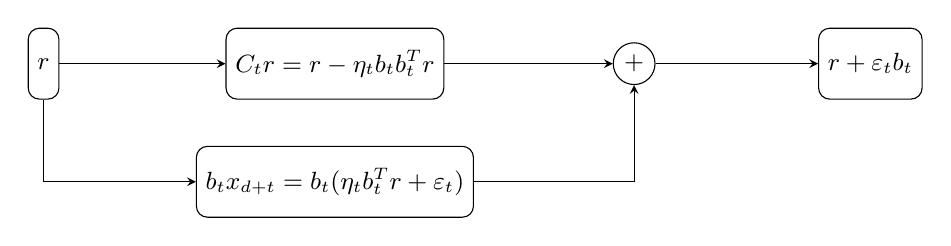
\begin{tikzpicture}[
   >=stealth,
   every node/.style={font=\small},
   state/.style={draw,rounded corners,align=center,minimum height=9mm}]
  \node[state] (r) at (0,0) {$r$};
  \node[state] (contract) at (3.7,0)
    {$C_tr=r-\eta_tb_tb_t^Tr$};
  \node[draw,circle,inner sep=2pt] (sum) at (7.5,0) {$+$};
  \node[state] (out) at (10.5,0) {$r+\varepsilon_tb_t$};
  \node[state] (incoming) at (3.7,-1.5)
    {$b_tx_{d+t}=b_t(\eta_tb_t^Tr+\varepsilon_t)$};
  \draw[->] (r) -- (contract);
  \draw[->] (contract) -- (sum);
  \draw[->] (sum) -- (out);
  \draw[->] (r.south) -- (0,-1.5) -- (incoming.west);
  \draw[->] (incoming.east) -- (7.5,-1.5) -- (sum.south);
 \end{tikzpicture}
\end{document}
